\chapter{Base teórica}\label{cap:teoria}
\section{Introdução}\label{sec:teoria_intro}
Dada a variedade de estudantes que podem ingressar em um curso de neurociência computacional, muitos deles podem não ter tido algumas disciplinas de base que são necessárias para um bom entendimento do conteúdo apresentado. Por isso, este capítulo contém uma base teórica útil para um nivelamento dos estudantes das mais diversas áreas. As sessões seguintes contemplam conteúdos de neurobiologia e equações diferenciais ordinárias. %, probabilidade e algoritmos.

\section{Neurobiologia básica}\label{sec:fisiologia}
O neurônio, mostrado na Figura~\ref{fig:neuronio}, é a unidade básica do sistema nervoso.
\begin{figure}[tb]
	\centering
	\caption[Neurônio]{Neurônio}
	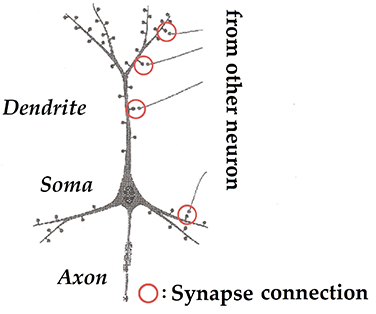
\includegraphics[width=0.55\linewidth]{figs/neuronio}
	\label{fig:neuronio}
	\fonte{Adaptado de \cite{lopez-ruiz_simulation_2016}}
	%TODO: trocar figura
\end{figure}
É composto pelo corpo celular (chamado de soma), dendritos, que recebem sinais de outros neurônios, axônio, que transmite os sinais a outros neurônios, e terminais axônicos, que são as extremidades do axônio e se conectam com os dendritos de outros neurônios. Como outras células do corpo humano, o neurônio é composto por íons e moléculas, ambos podendo possuir cargas positivas ou negativas. A célula neuronal é revestida por uma bi-camada lipídica, e geralmente o interior dela possui uma maior concentração de cargas negativas, fazendo com que o potencial de membrana ($V_m$), que é a diferença de potencial entre a parte interna e a externa da célula neuronal ($V_M=V_{dentro}-V_{fora}$), fique a maior parte do tempo com valor negativo. O potencial de membrana se altera quando há o fluxo de íons através dos poros de canais iônicos (Figura~\ref{fig:membrananeuronio}).

\begin{figure}[tb]
	\centering
	\caption[Membrana do neurônio]{Membrana do neurônio}
	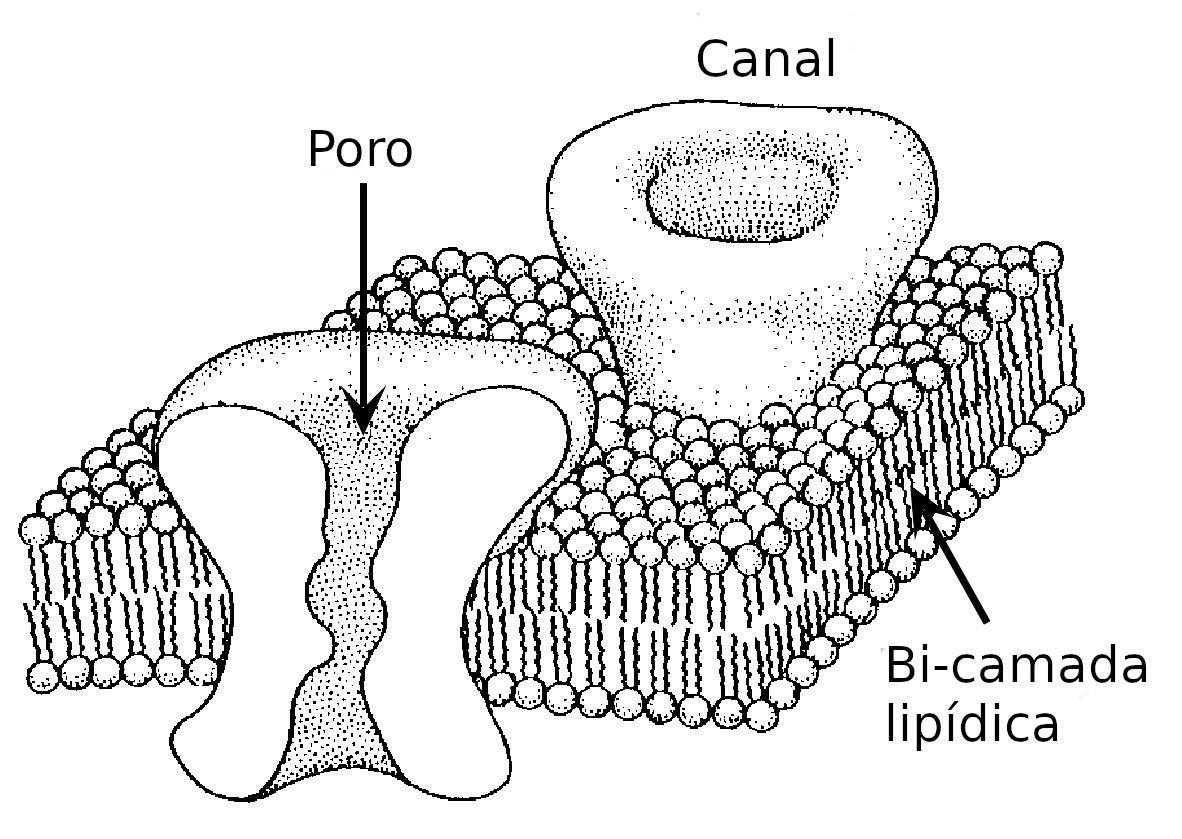
\includegraphics[width=0.55\linewidth]{figs/membrana_neuronio}
	\label{fig:membrananeuronio}
	\fonte{adaptado de \cite{hille_ionic_1992}}
\end{figure}

Os canais iônicos são canais proteicos na membrana da célula neuronal e permitem a movimentação de íons através deles, como mostrado na Figura~\ref{fig:canaisions}. Podem ser de dois tipos: com ou sem portão. Canais sem portão estão sempre abertos, enquanto os com portão podem abrir ou fechar, dependendo do valor do potencial de membrana, e por isso são chamados de canais iônicos dependentes de tensão. Quando o fluxo de corrente elétrica de todos os íons é equilibrado dentro e fora da célula neuronal (ou seja, o potencial de membrana não se altera), ele é chamado de potencial de repouso (ou de equilíbrio). O valor típico é próximo de $-70\ mV$. O valor do potencial de repouso ($E_A$) é calculado com base na concentração de cada íon dentro e fora da célula neuronal usando a equação de Nernst, dada por:
\begin{equation}\label{eq:nernst}
E_A=\frac{k_BT}{z_Aq_e}ln\left(\frac{A_{fora}}{A_{dentro}}\right)
\end{equation}
sendo $A$ o íon, $z_A$ a carga do íon, $A_{fora}$ e $A_{dentro}$ a concentração desse íon fora e dentro da célula neuronal, respectivamente, $T$ a temperatura absoluta (em Kelvin), $k_B$ a a constante de \textit{Boltzmann} ($1,39\text{x}10^{-23}\ JK^{-1}$) e $q_e$ a carga elétrica fundamental ($1,6\text{x}10^{-19}\ C$). Os valores de cargas, concentração e potencial de Nernst para alguns íons são apresentados na Tabela~\ref{tab:concentracao_nernst}.

\begin{figure}[tb!]
	\centering
	\caption[Canais iônicos de potássio]{Canais iônicos de potássio. Em \textbf{a} os íons de potássio saem da célula, causando um excesso de cargas positivas fora e negativas dentro. Em \textbf{b} o fluxo para fora e dentro é igual, causando equilíbrio}
	\label{fig:canaisions}
	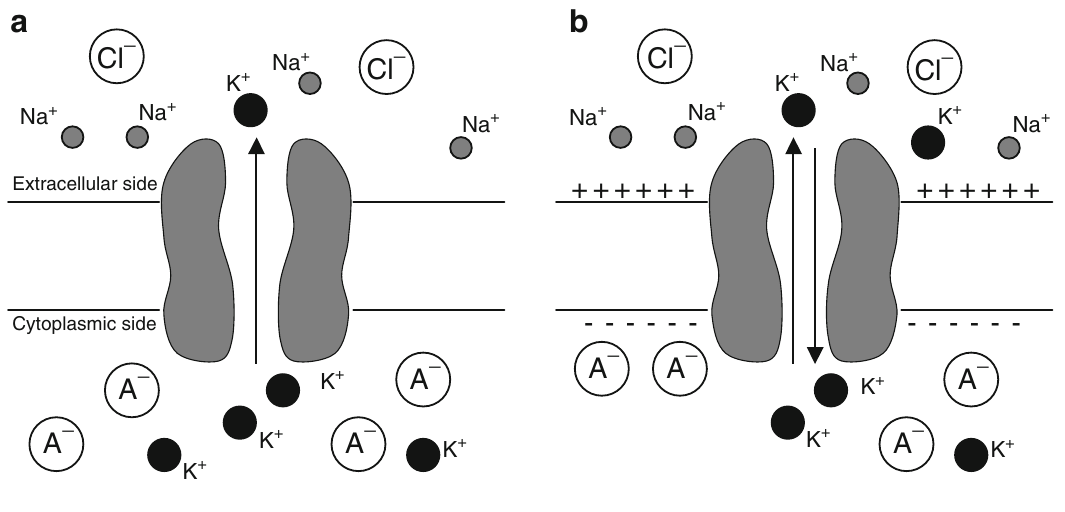
\includegraphics[width=0.7\linewidth]{figs/canais_ions}
	\fonte{Adaptado de \cite{ermentrout_mathematical_2010}}
\end{figure}

\begin{table}
	\IBGEtab{%
	\caption[Concentração de íons]{Concentração de íons}
	\label{tab:concentracao_nernst}
	}{%
	\begin{tabular}{c|c|c|c|c}
		\hline
		Íon & Carga & Conc. interna ($nM$) & Conc. externa ($nM$) & Potencial de reversão ($mV$) \\
		\hline
		Sódio & +1 & 15 & 120 & 61,6 \\
		\hline
		Potássio & +1 & 150 & 6 & -86,1 \\
		\hline
		Cloreto & -1 & 52 & 560 & -65 \\
		\hline
		Cálcio & +2 & 50 & 2 & 141,7 \\
		\hline
	\end{tabular}%
	}{
	\fonte{O autor (2023)}%
	}
\end{table}

Fora do repouso, a diferença de potencial entre o interior e o exterior do neurônio produz movimentação iônica. Quando íons positivos (como $Na^+$ ou $Ca^{2+})$ entram na célula neuronal, o potencial de membrana fica menos negativo (até próximo de 0 mV), fenômeno conhecido como despolarização. De maneira semelhante, quando íons positivos (como $K^+$) saem da célula neuronal, ou negativos (como $Cl^-$) entram, o potencial de membrana fica mais negativo, fenômeno conhecido como hiperpolarização. Os canais de potássio são mais presentes na membrana do neurônio, sendo os principais responsáveis pelo potencial de equilíbrio. Já os canais de sódio, associados à despolarização, são responsáveis pela geração do potencial de ação. Devido ao excesso de cargas negativas no interior da célula neuronal, e a existência de cargas positivas no exterior, a membrana do neurônio acaba funcionando como um capacitor, criando uma capacitância ($C_m$). O fluxo de íons através de canais sem portão é considerado constante, podendo ser agrupado em um elemento chamado de vazamento (\textit{leak}, em inglês), possuindo um potencial ($E_l$) e uma condutância ($G_l$), que é a facilidade desse elemento permitir o fluxo de corrente (o inverso da resistência). Com isso, é possível escrever uma equação relacionando o potencial de membrana da célula neuronal e os elementos de vazamento, como segue:
\begin{equation}\label{eq:potencial_membrana}
	\frac{\mathrm{d}V_m}{\mathrm{d}t}=G_l(E_l-V_m)/C_m
\end{equation}
que é dada na forma de uma equação diferencial, detalhada na seção seguinte.

\section{Equações diferenciais ordinárias}\label{sec:eqdif}
As equações diferenciais são usadas para descrever sistemas dinâmicos, ou seja, que se alteram ao longo do tempo. A forma mais básica de uma equação diferencial é:
\begin{equation}\label{eq:eq_diferencial}
	\frac{\mathrm{d}y(t)}{\mathrm{d}t}=F(t,y(t))
\end{equation}
com o lado esquerdo da equação sendo a derivada de $y(t)$, a função presente no lado direito associada à variável $t$, que geralmente representa o tempo, e $F$ representando uma função qualquer com $t$ e $y$. Diferentemente das equações algébricas, que possuem como solução um número, as equações diferenciais tem uma família de funções como solução, variando de acordo com a escolha de constantes, como mostrado na Figura~\ref{fig:solucao}. Nela, é exibida a família de soluções $y(t) = t + 1 + ce^t$ para a equação diferencial $y'=y-t$. $y'$ é uma representação equivalente para $\frac{\mathrm{d}y(t)}{\mathrm{d}t}$. Qualquer valor de $c$ real que for escolhido representa uma solução possível para a equação, sendo exibidas as curvas para os valores de $c$ iguais a $0$, $-1$ e $0,4$.

\begin{figure}[tb]
	\centering
	\caption{Soluções $y(t) = t + 1 + ce^t$ da equação $y'=y-t$ para vários valores de $c$}
	\label{fig:solucao}
	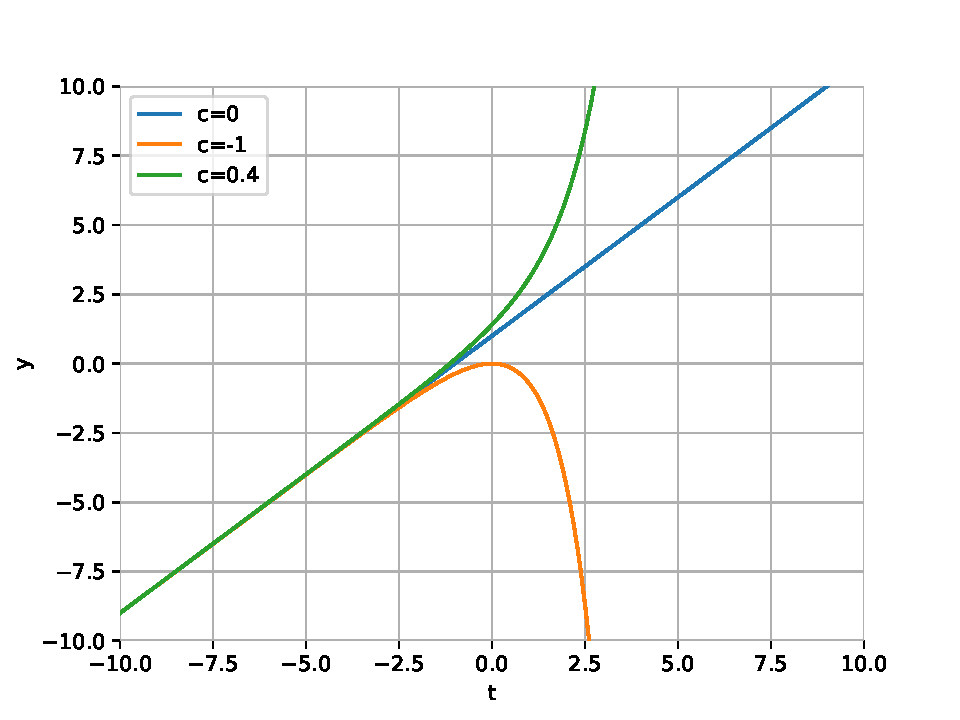
\includegraphics[width=0.7\linewidth]{figs/solucao}
	\fonte{O autor (\the\year)}
\end{figure}


\subsection{Exemplos}
\subsubsection{Decaimento radioativo}
Segundo a lei do decaimento radioativo, a taxa na qual os átomos radioativos se desintegram é proporcional ao número total de átomos radioativos presente. Sendo $N(t)$ o número de átomos radioativos no tempo $t$, então $N'(t)$ é a taxa de mudança. A lei do decaimento radioativo é a que segue:
\begin{equation}\label{eq:decaimento_radioativo}
	N'(t) = -\lambda N(t)
\end{equation}
onde $\lambda$ é a constante de decaimento. O gráfico de uma possível solução para essa equação diferencial é exibido na Figura~\ref{fig:decaimento}.

\begin{figure}[tb]
	\centering
	\caption{Decaimento radioativo ($\lambda = 0,5$)}
	\label{fig:decaimento}
	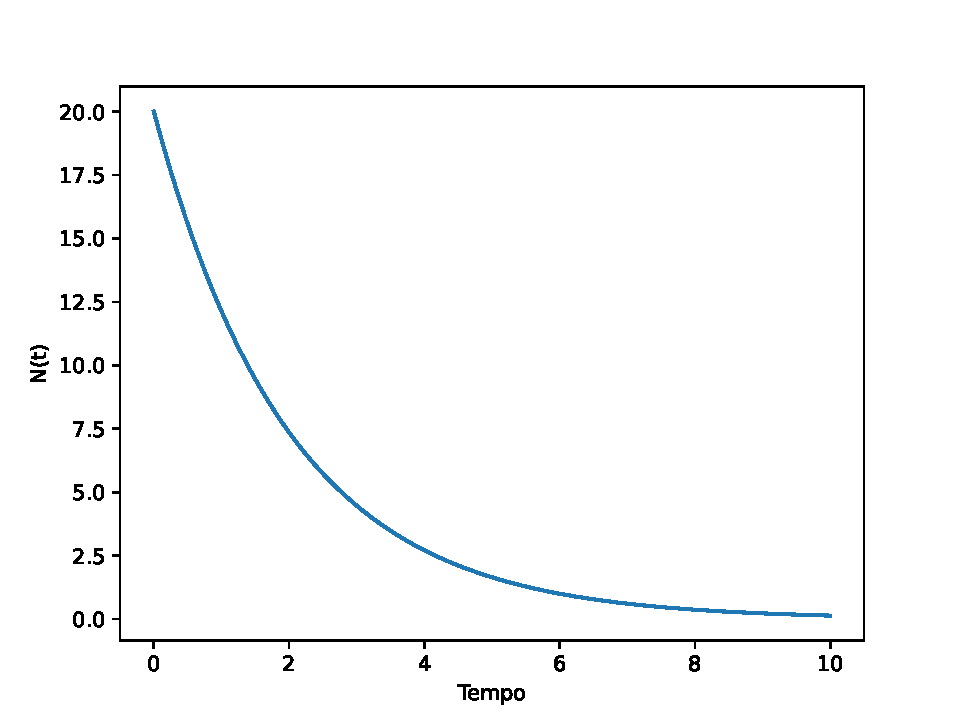
\includegraphics[width=0.6\linewidth]{figs/decaimento}
	\fonte{O autor (\the\year)}
\end{figure}

\subsubsection{Equações de Lotka-Volterra}
Também conhecidas como equações predador-presa, são um par de equações diferenciais de primeira ordem, frequentemente usadas para descrever a dinâmica de sistemas biológicos de interação entre duas espécies, uma como predadora e a outra como presa. As populações de cada uma das espécies são dadas pelo par de equações:
\begin{equation}\label{eq:lotka_volterra}
	x' = ax - bxy
	$$$$
	y' = dxy - cy
\end{equation}
sendo $x$ a população da presa, $y$ a do predador, $x',\ y'$ as taxas de variação de cada população, e $a,\ b,\ c,\ d$ os parâmetros que descrevem a interação entre as espécies. A Figura~\ref{fig:lotka-volterra} exibe a solução do par de equações para um valor de cada parâmetro de interação.

\begin{figure}[tb]
	\centering
	\caption{Sistema de Lotka-Volterra ($a$ = 1,5; $b$ = 1; $c$ = 3; $d$ = 1)}
	\label{fig:lotka-volterra}
	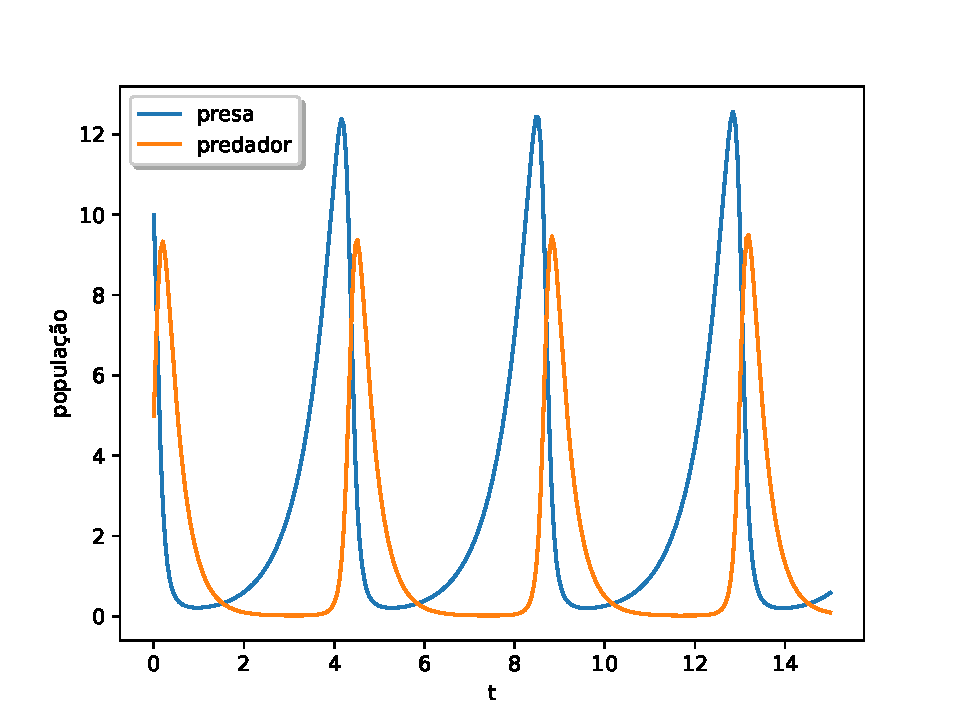
\includegraphics[width=0.6\linewidth]{figs/lotka-volterra}
	\fonte{O autor (\the\year)}
\end{figure}

\subsection{Método de Euler}
Equações diferenciais ordinárias podem ser resolvidas analiticamente, não abordado neste texto, ou numericamente. Dentre os vários métodos existentes para a solução numérica, a adotada aqui é o método de Euler. Considerando a equação $\frac{dx}{dt}=f(x,t)$, com $f(x,t)$ uma função qualquer de $x$ em relação a $t$, dado um valor inicial $x0$ (usualmente com $t=0$), é possível simular a equação usando pontos discretos com intervalos $\Delta t$ fixos. Cada valor $x_n$ é dado por $x_n=x(t_n=n\Delta t)$. A partir disso, é possível usar o método de Euler avançado para calcular um valor seguinte a partir do valor anterior, ou seja:
$$
x_{n+1}=x_n+f(x_n,t_n)\Delta t
$$
como é demonstrado na Figura~\ref{fig:euler}. Outros métodos não abordados no curso incluem o método de Euler reverso e o Runge-Kutta de segunda e quarta ordens, que são mais precisos na solução. O algoritmo (sequência de instruções para executar uma determinada tarefa) do método de Euler será implementado usando a linguagem Python, que tem a sua base detalhada no Apêndice~\ref{ap:python}.
\begin{figure}[tb]
	\centering
	\caption{Método de Euler}
	\label{fig:euler}
	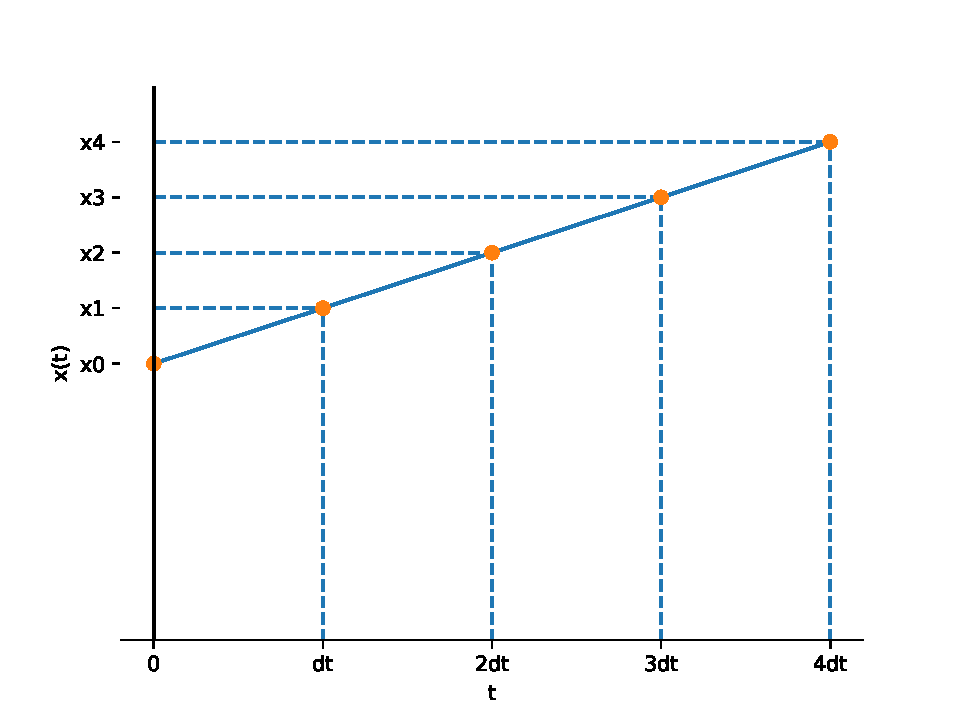
\includegraphics[width=0.7\linewidth]{figs/euler}
	\fonte{O autor (\the\year)}
\end{figure}
